\documentclass{beamer}
\usetheme{Montpellier}
\usecolortheme{dolphin}

%\usepackage{graphicx} %For jpg figure inclusion
%\usepackage{times} %For typeface
%\usepackage{epsfig}
\usepackage{color} %For Comments
\usepackage{beamerthemeshadow} %Paul and Lemmon put this in, take out if you want
%\usepackage[all]{xy}
%\usepackage{float}
%\usepackage{subfigure} 
%\usepackage{hyperref}
%\usepackage{url}
%\usepackage{parskip}
%\usepackage{multirow}

%% Elena's favorite green (thanks, Fernando!)
\definecolor{ForestGreen}{RGB}{34,139,34}
% Uncomment this if you want to show work-in-progress comments
\newcommand{\comment}[1]{{\bf \tt  {#1}}}
% Uncomment this if you don't want to show comments
%\newcommand{\comment}[1]{}
\newcommand{\emcomment}[1]{\textcolor{ForestGreen}{\comment{Elena: {#1}}}}
%%%%%%%%%%%%%%%%%%%%%%%%%%%%%%%%%%%%%%%%%%

\begin{document}
\title{Discussion about inclusiveness in CSci}
\author{UMM CSci}
\date{October 5, 2015}

\begin{frame}
\maketitle
\end{frame}

\begin{frame}
\frametitle{Why talk about inclusiveness?}
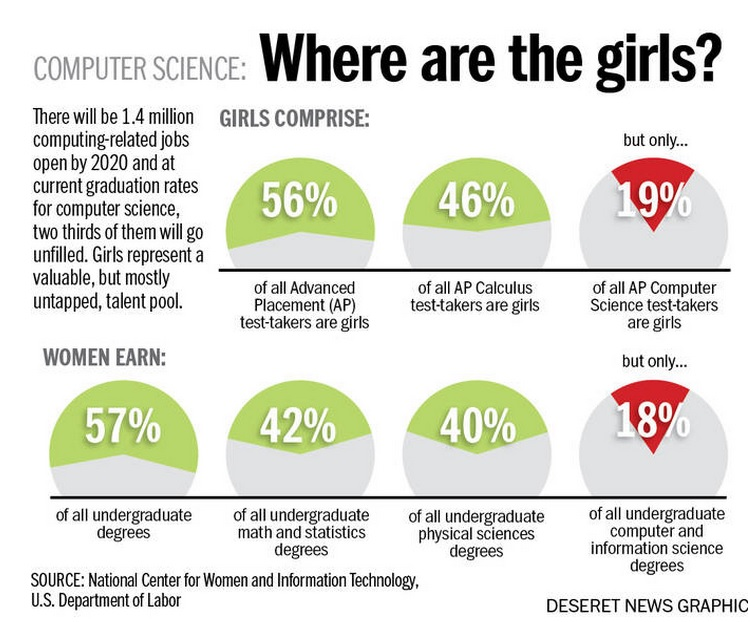
\includegraphics[scale=0.5]{Stats.jpg}
\end{frame}

\begin{frame}
\frametitle{Two videos}
What is the issue? 

{\it 
\href{https://www.youtube.com/watch?v=fQyCBTDproE}{The Underrepresentation of Women in STEM, by Chelsea Ziadle}}

A story of a woman engineer:

{\it
\href{https://www.youtube.com/watch?v=FEeTLopLkEo}{Inspiring the next generation of female engineers: Debbie Sterling at TEDxPSU}}

Similar problems are faced by ethnic minorities or anyone else who doesn't look like a stereotypical engineer. 
\end{frame}



\end{document}